\documentclass[pdf, aspectratio=169]{beamer}
\usepackage[]{hyperref,graphicx,siunitx,lmodern,booktabs,tikz,tensor}
\usepackage{pgfplots, pgfplotstable}
\usepackage{pdfpc-commands}

\usepackage[mode=buildnew]{standalone}
\mode<presentation>{\usetheme{Astro}}

\graphicspath{ {../Images/} }

\sisetup{per-mode=symbol}
\usetikzlibrary{calc,intersections, decorations.pathmorphing,shadings}
\tikzstyle{proton}=[circle, minimum size = 7mm, ball color=red, black,transform shape]
\tikzstyle{neutron}=[circle, minimum size=7mm, ball color=gray, black, transform shape]
\tikzstyle{gammaray}=[ultra thick, -latex, decorate, decoration={snake, post length=3mm}]


%preamble
\title{The Heavy Hitters}
\date{November 7, 2018}
\author{Jed Rembold}

\begin{document}
\renewcommand*{\theenumi}{\Alph{enumi}}

\begin{frame}{Announcements}
  \begin{itemize}
	\item Webwork due on Friday
	\item Test 3 one week from Friday!
		\begin{itemize}
			\item I'll aim to have study materials and old tests up by this weekend
			\item Our Sun through stars
			\item Probably finish content on Monday
		\end{itemize}
	\item Polling: \url{rembold-class.ddns.net}
  \end{itemize}
\end{frame}

\begin{frame}{A bit of review\ldots}
	A friend is telling you about main sequence stars they have been observing of different masses, a few of which include a $0.03 M_\odot$, $0.5 M_\odot$, $1 M_\odot$,and a $120 M_\odot$ star. Which would you be most skeptical about?
  \begin{enumerate}
	  \item \alert<2>{$0.03M_\odot$}
	  \item $0.5M_\odot$
	  \item $1M_\odot$
	  \item $120M_\odot$
  \end{enumerate}
\end{frame}

\begin{frame}{A Massive Undertaking}
  \begin{itemize}
	\item A star's mass is likely its most influential property
	\item Determines:
	  \begin{itemize}
		\item Luminosity
		\item Temperature
		\item Lifetime
		\item \alert{And its ultimate fate!}
	  \end{itemize}
	\item Catagorize:
	  \begin{itemize}
		\item \textcolor{orange}{Low-mass:} stars born with a mass $<2M_\odot$
		\item \textcolor{orange}{Intermediate-mass:} stars born with mass between $2$ and $8$ $M_\odot$
		\item \textcolor{orange}{High-mass:} stars born with mass $>8 M_\odot$
	  \end{itemize}
	\item<2> \alert{We'll look at low mass star lifetimes first, then look at intermediate and high mass lifetimes together}
  \end{itemize}
\end{frame}

\begin{frame}{The Main Sequence}
  \begin{columns}
	\column{.5\textwidth}
	\begin{itemize}
	  \item Happily creating energy by fusing hydrogen into helium
	  \item Equilibrium between gravity and gas pressure
	  \item Balanced between energy created and energy released
	  \item Provides a steady source of energy
	  \item Spends about 90\% of its total lifetime on the main sequence
		\begin{itemize}
		  \item Billions of years
		\end{itemize}
	\end{itemize}
	\column{.5\textwidth}
	\begin{center}
	  \includegraphics[width=.9\textwidth]{ch13_sun.jpg}
	\end{center}
  \end{columns}
\end{frame}

\begin{frame}{A Fateful Day}
  \begin{itemize}
	\item We feel fairly decent at this point about the main sequence
	\item Our key question is what happens after that?
	\item Linked to running out of hydrogen to fuse, but \alert{what does that imply for our star?}
  \end{itemize}
\end{frame}

\begin{frame}{A Delicate Balance\ldots}
  \begin{columns}
	\column{.5\textwidth}
	\begin{itemize}
	  \item The core runs out of hydrogen
		\begin{itemize}
		  \item Gas pressure lessens $\Rightarrow$ gravity wins
		  \item Core compresses
		\end{itemize}
	  \item<2-> Outer layers still have hydrogen
	  \item<2-> Core contraction brings the innermost of these layers into the ``fusing zone''
	  \item<2-> Hydrogen shell actually ``burns hotter''!
	\end{itemize}
	\column{.5\textwidth}
	\begin{tikzpicture}
	  \shade[inner color=yellow, outer color=Background, even odd rule] (0,0) circle (2cm) (0,0) circle (3cm);
	  \fill[orange!50!yellow] (0,0) circle (2cm);

	  \fill<1>[red] (0,0) circle (5mm);
	  \fill<2->[red] (0,0) circle (3mm);
	  \draw<2->[red,dashed] (0,0) circle (5mm);
	\end{tikzpicture}
  \end{columns}
\end{frame}

\begin{frame}{A Broken Thermostat\ldots}
  \begin{columns}
	\column{.5\textwidth}
	\begin{itemize}
	  \item Increase of fusion rate releases lots more energy
		\begin{itemize}
		  \item Increases gas pressure
		  \item Outer layers puff up
		  \item Solar winds start blowing away material
		\end{itemize}
	  \item<2-> As the hydrogen shell fuses, its helium is added to the core
		\begin{itemize}
		  \item Increased mass compresses it further
		  \item New shell burns even hotter
		  \item Outer layers puff up more
		\end{itemize}
	\end{itemize}
	\column{.5\textwidth}
	\begin{tikzpicture}
	  \shade[inner color=yellow, outer color=Background, even odd rule] (0,0) circle (2cm) (0,0) circle (3cm);
	  \fill[orange!50!yellow] (0,0) circle (2.5cm);
	  \fill<3->[orange!50!yellow] (0,0) circle (3cm);

	  \fill<1>[red] (0,0) circle (3mm);
	  \draw<1>[red,dashed] (0,0) circle (5mm);
	  \draw[dashed,orange] (0,0) circle (2.3cm);
	  
	  \fill<2->[red] (0,0) circle (1mm);
	  \draw<2->[red,dashed] (0,0) circle (3mm);
	\end{tikzpicture}
  \end{columns}
\end{frame}

\begin{frame}[fragile]{Helium Fusion!}
  \begin{itemize}
	\item At temperatures of about 100 million K, helium starts fusing to Carbon
	  \begin{itemize}
		\item Uses a two step process
		\item Need such high temperatures because \nuclide[8]{Be} is very unstable
		\item Need it to combine with another Helium before it decays
	  \end{itemize}
	\item Helium fusion actually causes the star to shrink some in size!
	\item Some Oxygen also created (adding another Helium to Carbon)
  \end{itemize}
  \newcommand{\helium}[2]{
	\begin{scope}[#2]
	  \coordinate (c) at (#1);
	  \node[proton] at ($(c)-(3.5mm,0)$) {p};
	  \node[proton] at ($(c)+(3.5mm,0)$) {p};
	  \node[neutron] at ($(c)+(0,3.5mm)$) {n};
	  \node[neutron] at ($(c)-(0,3.5mm)$) {n};
	\end{scope}
  }
  \begin{center}
	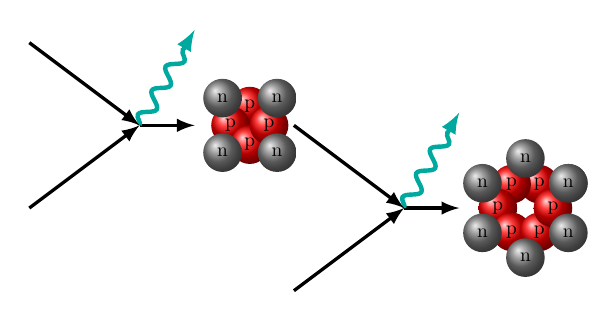
\begin{tikzpicture}[scale=.7]
	  \helium{0,0}{};
	  \helium{0,-3}{};

	  \onslide<2->{
		\coordinate (Be) at (5,-1.5);
		\foreach \p in {1,2,3,4}{
		  \node[proton] at ($(Be)+({90*\p}:3.5mm)$) {p};
		}
		\foreach \n in {0,1,2,3}{
		  \node[neutron] at ($(Be)+({45+90*\n}:7mm)$) {n};
		}
		\draw[very thick, latex-] ($(Be)-(1,0)$) --+(-1,0) coordinate (exp);
		\draw[gammaray, cyan!50!green] (exp) --+(60:2);
		\draw[very thick, latex-] (exp) --+(-2,1.5);
		\draw[very thick, latex-] (exp) --+(-2,-1.5);
	  }

	  \onslide<3->{
		\helium{5,-4.5}{};
		\coordinate (C) at (10,-3);
		\foreach \p in {1,2,...,6}{
		  \node[proton] at ($(C)+({60*\p}:5mm)$) {p};
		}
		\foreach \n in {0,1,...,6}{
		  \node[neutron] at ($(C)+({30+60*\n}:9mm)$) {n};
		}
		\draw[very thick, latex-] ($(C)-(1.2,0)$) --+(-1,0) coordinate (exp);
		\draw[gammaray, cyan!50!green] (exp) --+(60:2);
		\draw[very thick, latex-] (exp) --+(-2,1.5);
		\draw[very thick, latex-] (exp) --+(-2,-1.5);
	  }
	\end{tikzpicture}
  \end{center}
\end{frame}

\begin{frame}{A Flash in the Pan}
  \begin{columns}
	\column{.5\textwidth}
	\begin{itemize}
	  \item Energy from initial helium fusion rapidly expands core (Helium Flash)
		\begin{itemize}
		  \item Pushes out hydrogen burning shell
		\end{itemize}
	  \item<2-> Star actually shrinks some and warms back up
	  \item<3-> Reaches stability and undergoes helium fusion
		\begin{itemize}
		  \item Lasts maybe 10-20\% as long as hydrogen fusion
		\end{itemize}
	  \item<4-> When run out of helium, a repeat occurs, but even worse
	\end{itemize}
	\column{.5\textwidth}
	\begin{tikzpicture}
	  \shade[inner color=yellow, outer color=Background, even odd rule] (0,0) circle (2cm) (0,0) circle (3cm);
	  \fill<1,2>[orange!50!yellow] (0,0) circle (3cm);
	  \fill<3->[orange!50!yellow] (0,0) circle (2.25cm);
	  \fill<1>[red] (0,0) circle (1mm);
	  \draw<1->[red,dashed] (0,0) circle (3mm);
	  \fill<2->[red] (0,0) circle (2mm);
	  \fill<3>[red!50!black] (0,0) circle (0.5mm);
	  \fill<4>[red!50!black] (0,0) circle (1mm);
	\end{tikzpicture}
  \end{columns}
\end{frame}

\begin{frame}{Game Over}
  \begin{itemize}
	\item What happens when the star runs out of helium?
	\item Another growth surge:
	  \begin{itemize}
		\item Core cools, and constricts
		\item Now there are two fusing shells, one of helium and one of hydrogen
		\item Heats outer layers and causes star to puff up even bigger!
	  \end{itemize}
	\item Core collapses inward until supported by degeneracy pressure
	\item Not massive enough to squeeze carbon atoms close enough together to start carbon fusion
	\item Internal energy source turns off
	\item Most gas outside the core has been blown away
	\item Becomes a white dwarf
	\item Outgoing radiation excites expelled gases, creating planetary nebula!
  \end{itemize}
\end{frame}

\fullFrameImage{ch13_planetary_nebula.png}

\begin{frame}{Understanding Check}
  Which of the following HR Diagrams would show the path of our Sun's lifetime?
  \begin{center}
	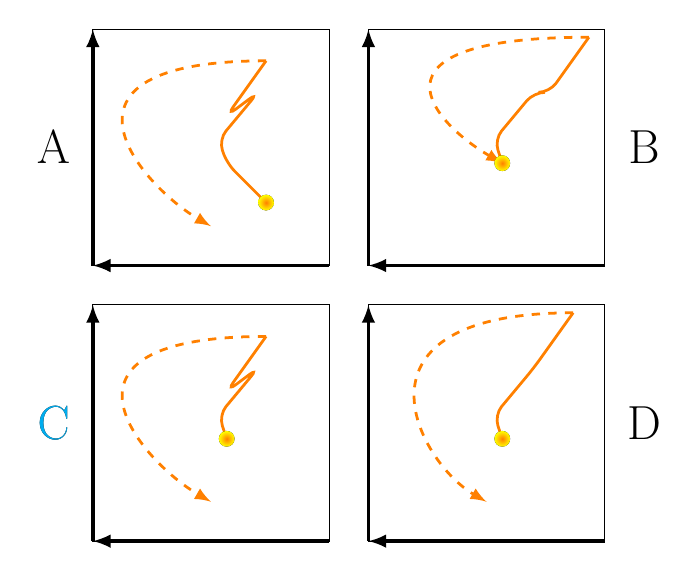
\begin{tikzpicture}
	  \coordinate (A) at (0,0);
	  \draw (A) rectangle +(3,3);
	  \draw[very thick, -latex] (A) --+(0,3);
	  \draw[very thick, latex-] (A) --+(3,0);
	  \coordinate (start) at ($(A)+(1.7,1.3)$);
	  \draw[line width=1pt, orange, rounded corners] (start) --++(-.1,.3) --++(.5,.6) --++(-.4,-.3) --++(.5,.7) coordinate (end);
	  \draw[line width=1pt, dashed, orange, -latex] (end) .. controls +(180:3) and +(150:1) .. ($(A)+(1.5,.5)$);
	  \fill[inner color=orange, outer color=yellow] (start) circle (1mm);
	  \node at ($(A)+(-.5,1.5)$) {\LARGE C};
	  \node<2>[cyan] at ($(A)+(-.5,1.5)$) {\LARGE C};

	  \coordinate (A) at (3.5,0);
	  \draw (A) rectangle +(3,3);
	  \draw[very thick, -latex] (A) --+(0,3);
	  \draw[very thick, latex-] (A) --+(3,0);
	  \coordinate (start) at ($(A)+(1.7,1.3)$);
	  \draw[line width=1pt, orange, rounded corners] (start) --++(-.1,.3) --++(.5,.6) --++(.5,.7) coordinate (end);
	  \draw[line width=1pt, dashed, orange, -latex] (end) .. controls +(180:3) and +(150:1) .. ($(A)+(1.5,.5)$);
	  \fill[inner color=orange, outer color=yellow] (start) circle (1mm);
	  \node at ($(A)+(3.5,1.5)$) {\LARGE D};

	  \coordinate (A) at (0,3.5);
	  \draw (A) rectangle +(3,3);
	  \draw[very thick, -latex] (A) --+(0,3);
	  \draw[very thick, latex-] (A) --+(3,0);
	  \coordinate (start) at ($(A)+(1.7,1.3)$);
	  \draw[line width=1pt, orange, rounded corners] (start)+(.5,-.5)--(start) --++(-.1,.3) --++(.5,.6) --++(-.4,-.3) --++(.5,.7) coordinate (end);
	  \draw[line width=1pt, dashed, orange, -latex] (end) .. controls +(180:3) and +(150:1) .. ($(A)+(1.5,.5)$);
	  \fill[inner color=orange, outer color=yellow] ($(start)+(.5,-.5)$) circle (1mm);
	  \node at ($(A)+(-.5,1.5)$) {\LARGE A};

	  \coordinate (A) at (3.5,3.5);
	  \draw (A) rectangle +(3,3);
	  \draw[very thick, -latex] (A) --+(0,3);
	  \draw[very thick, latex-] (A) --+(3,0);
	  \coordinate (start) at ($(A)+(1.7,1.3)$);
	  \draw[line width=1pt, orange, rounded corners] (start) --++(-.1,.3) --++(.5,.6) --++(.2,0) --++(.5,.7) coordinate (end);
	  \draw[line width=1pt, dashed, orange, -latex] (end) .. controls +(180:3) and +(150:1) .. (start);
	  \fill[inner color=orange, outer color=yellow] (start) circle (1mm);
	  \node at ($(A)+(3.5,1.5)$) {\LARGE B};
	\end{tikzpicture}
  \end{center}
\end{frame}

\begin{frame}{Time to get Massive}
  \begin{itemize}
	\item Now we'll shift our attention to the more massive stars
	\item Talking stars with masses greater that $2M_\odot$
  \end{itemize}
  \begin{center}
	\includegraphics[width=.55\textwidth]{ch13_crab.jpg}
  \end{center}
\end{frame}

\begin{frame}{The Boring Part}
  \begin{columns}
	\column{.5\textwidth}
	\begin{itemize}
	  \item Like their low mass bretheren, high mass stars start out on the main sequence
	  \item Burning hydrogen
	  \item Larger mass means:
		\begin{itemize}
		  \item Blue (Hotter)
		  \item Brighter (Greater Luminosity)
		\end{itemize}
	  \item Fuses through a CNO cycle instead of Proton-Proton chains
	\end{itemize}
	\column{.6\textwidth}
	\begin{center}
	  \begin{tikzpicture}
		\pgfplotsset{colormap={stars}{[0.1cm] color(0cm)=(blue); color(1.8cm)=(white); color(2.1cm)=(yellow); color(2.6cm)=(red); color(3cm)=(red!50!black)}}
		\hspace{-1cm}
		\begin{loglogaxis}[
			width=7.5cm,
			height=7.5cm,
			x dir = reverse,
			%xlabel = Temperature (K),
			%ylabel = Fraction of Sun's Luminosity,
			ticklabel style={font=\tiny},
			xtick = {3000, 6000, 10000, 25000},
			xticklabels = {3000,6000,10000,25000},
			colormap name= stars,
			xmin = 2000,
			xmax = 40000,
		  ]
		  \addplot[scatter, scatter src=-x, draw=black, only marks, mark size = 1pt] table[x index=0, y index=1] {../Data/HR_Data.csv};
		  \node at (axis cs: 10^4.5,10^-4) {O};
		  \node at (axis cs: 10^4.2,10^-4) {B};
		  \node at (axis cs: 10^3.95,10^-4) {A};
		  \node at (axis cs: 10^3.85,10^-4) {F};
		  \node at (axis cs: 10^3.7,10^-4) {G};
		  \node at (axis cs: 10^3.6,10^-4) {K};
		  \node at (axis cs: 10^3.4,10^-4) {M};
		\end{loglogaxis}
		\draw<2>[cyan, ultra thick] (1.4,4.2) circle (1.5cm);
	  \end{tikzpicture}
	\end{center}
  \end{columns}
\end{frame}

\begin{frame}{The CNO Cycle}
  \begin{center}
	\includegraphics[width=.56\textwidth]{ch13_CNO_Cycle.pdf}
  \end{center}
\end{frame}

\begin{frame}{When the H runs out\ldots}
  \begin{itemize}
	\item The hotter temperatures and CNO cycle fuse the hydrogen much quicker than in low mass stars
	\item The effects of running out of hydrogen in the core is similar to low mass stars:
	  \begin{itemize}
		\item The core begins to cool and contract
		\item Hydrogen shell burning begins and puffs out the outer layers
		\item The core contracts and heats until hot enough for helium fusion
	  \end{itemize}
	\item Becomes a \alert{Supergiant!}
	\item When Helium fusion activates, there is no helium flash
	  \begin{itemize}
		\item Core still hot enough to support with gas pressure
	  \end{itemize}
	\item Outer layers slower to react means the luminosity stays about the same
  \end{itemize}
\end{frame}

\begin{frame}{When the (Insert Element Here) runs out\ldots}
  \begin{itemize}
	\item Things get exciting!
	\item Core contracts again
	  \begin{itemize}
		\item This time there \alert{is} enough mass and heat to start carbon fusion
		\item Repeats the same cycle as with helium fusion
		\item But even shorter timescales this time
		\item Carbon fuses into Neon, Sodium, and Magnesium
	  \end{itemize}
	\item Then the carbon runs out!
	  \begin{itemize}
		\item Core contracts again until hot enough for Oxygen or Neon fusion to begin
	  \end{itemize}
	\item Cycle keeps repeating each time the core runs out of fuel
	  \begin{itemize}
		\item Each cycle results in larger elements being produced
		\item Each cycle is shorter, as there is less of the heavier element
		\item At some point we reach Iron
	  \end{itemize}
  \end{itemize}
\end{frame}

\begin{frame}{Our Onion Star}
  At this point we have multiple layers of shell fusion happening throughout the star
  \begin{center}
	\begin{tikzpicture}[scale=.8, lbl/.style={minimum width=2cm, minimum height=.75cm, anchor=west}]
	  \shade[inner color=yellow, outer color=Background, even odd rule] (0,0) circle (2cm) (0,0) circle (4cm);
	  \fill[orange!50!yellow] (0,0) circle (3.5cm);
	  \fill[red] (0,0) circle (2cm);
	  \fill[red!50!black] (0,0) circle (1cm);
	  \fill[blue!70!black] (0,0) circle (5mm);
	  \fill[green!50!black] (0,0) circle (2mm);
	  \fill[gray!50!black] (0,0) circle (1mm);

	  \node[fill=orange!50!yellow,lbl, text=black] at (4.5,2.5) {Hydrogen};
	  \node[fill=red,lbl, text=black] at (4.5,1.5) {Helium};
	  \node[fill=red!50!black, lbl] at (4.5,.5) {Carbon};
	  \node[fill=blue!70!black, lbl] at (4.5,-.5) {Oxygen};
	  \node[fill=green!50!black, lbl, text=black] at (4.5,-1.5) {Silicon};
	  \node[fill=gray!50!black, lbl] at (4.5,-2.5) {Iron};
	\end{tikzpicture}
  \end{center}
\end{frame}

%\begin{frame}{Iron: The Great Killjoy \scriptsize Or is it!?}
  %\begin{columns}
	%\column{.5\textwidth}
	%\begin{center}
	  %\begin{tikzpicture}
		%\begin{axis}[
			%width=6.5cm,
			%height=7cm,
			%xlabel = Mass Number (Neutrons + Protons),
			%ylabel = Binding Energy (MeV),
			%ylabel near ticks,
		  %]
		  %\addplot[scatter] table {../Data/BindingEnergy.csv};
		  %\node[pin=-90:Iron] at (axis cs: 56,8.5) {};
		  %\node[pin=45:Hydrogen] at (axis cs: 1,1) {};
		  %\node[pin=250:Uranium] at (axis cs: 238,7.3) {};
		%\end{axis}
	  %\end{tikzpicture}
	%\end{center}
	%\column{.5\textwidth}
	%\begin{itemize}
	  %\item Fusing elements greater than iron \alert{uses} energy!
	  %\item Iron also sucks up loose electrons running around
		%\begin{itemize}
		  %\item Decreases the internal electron degeneracy pressure
		%\end{itemize}
	  %\item Basically, once the star hits iron, it's game over
		%\begin{itemize}
		  %\item At least for fusion
		  %\item For other things, it's party time
		%\end{itemize}
	%\end{itemize}
  %\end{columns}
%\end{frame}

%\begin{frame}{Party Time!}
  %\begin{itemize}
	%\item Impossible for the core to contract enough to fuse iron and give off energy
	%\item Can electron degeneracy stop the collapse? (Like with brown and white dwarfs?)
	  %\begin{itemize}
		%\item NOPE! Too much mass!
		%\item Physics laws can't be violated:
		  %\begin{itemize}
			%\item All electrons combine with protons to make neutrons + neutrinos
		  %\end{itemize}
		%\item Pure neutron core continues to collapse
		%\item Can neutron degeneracy pressure stop the collapse?
		  %\begin{itemize}
			%\item Maybe!
		  %\end{itemize}
	  %\end{itemize}
	%\item The collapse is incredibly violent
	%\item Neutrinos from the creation of the neutrons surge outward with ridiculous energies
	%\item So dense and so many that they actually interact with the surrounding gas, exploding it outward
  %\end{itemize}
%\end{frame}

%\begin{frame}{Supernova Details}
  %\begin{itemize}
	%\item Core with mass of Sun and size of Earth contracts
	  %\begin{itemize}
		%\item Final size? A few kilometers across
		%\item Time to collapse? A fraction of a second
	  %\end{itemize}
	%\item Radiates 100 times the energy that the Sun will radiate \alert{over its entire 10 billion year lifetime}
	%\item The immense heat excites the gas that is exploding outward, causing it to shine
	%\item The insane pressure and energy also give elements heavier than iron a chance to form
	  %\begin{itemize}
		%\item Without supernovae, we wouldn't exist!
	  %\end{itemize}
  %\end{itemize}
%\end{frame}

%\fullFrameMovie{../Videos/Crab_Explosion.ogv}{../Videos/Crab_Explosion.png}

%\begin{frame}{Supernova Prettiness}
  %\begin{center}
	%\begin{tikzpicture}[image/.style={inner sep=0pt, outer sep=0pt, anchor=south west}]
	  %\node[image] at (0,0) {\includegraphics[width=6cm]{ch13_crab.jpg}};
	  %\node[image] at (5.5,1) {\includegraphics[width=5cm]{ch13_SN1994D.jpg}};
	  %\node[image, anchor=north west] at (10,2.5) {\includegraphics[width=4cm]{ch13_cassA.jpg}};
	%\end{tikzpicture}
  %\end{center}
%\end{frame}

%\begin{frame}{Binary Complications}
  %\begin{itemize}
	%\item Happy orbit each other during main sequence
	%\item When one goes Giant, suddenly the other can start stealing its mass!
	%\item Accelerates the life-cycle of the thief
  %\end{itemize}
  %\begin{center}
	%\includegraphics[width=.5\textwidth]{ch13_mass_transfer.jpg}
  %\end{center}
%\end{frame}




\end{document}
